\RequirePackage{atbegshi}
\documentclass[compress,aspectratio=169]{beamer}\usepackage[]{graphicx}\usepackage[dvipsnames]{xcolor}
% maxwidth is the original width if it is less than linewidth
% otherwise use linewidth (to make sure the graphics do not exceed the margin)
\makeatletter
\def\maxwidth{ %
  \ifdim\Gin@nat@width>\linewidth
    \linewidth
  \else
    \Gin@nat@width
  \fi
}
\makeatother

\definecolor{fgcolor}{rgb}{0.345, 0.345, 0.345}
\newcommand{\hlnum}[1]{\textcolor[rgb]{0.686,0.059,0.569}{#1}}%
\newcommand{\hlsng}[1]{\textcolor[rgb]{0.192,0.494,0.8}{#1}}%
\newcommand{\hlcom}[1]{\textcolor[rgb]{0.678,0.584,0.686}{\textit{#1}}}%
\newcommand{\hlopt}[1]{\textcolor[rgb]{0,0,0}{#1}}%
\newcommand{\hldef}[1]{\textcolor[rgb]{0.345,0.345,0.345}{#1}}%
\newcommand{\hlkwa}[1]{\textcolor[rgb]{0.161,0.373,0.58}{\textbf{#1}}}%
\newcommand{\hlkwb}[1]{\textcolor[rgb]{0.69,0.353,0.396}{#1}}%
\newcommand{\hlkwc}[1]{\textcolor[rgb]{0.333,0.667,0.333}{#1}}%
\newcommand{\hlkwd}[1]{\textcolor[rgb]{0.737,0.353,0.396}{\textbf{#1}}}%
\let\hlipl\hlkwb

\usepackage{framed}
\makeatletter
\newenvironment{kframe}{%
 \def\at@end@of@kframe{}%
 \ifinner\ifhmode%
  \def\at@end@of@kframe{\end{minipage}}%
  \begin{minipage}{\columnwidth}%
 \fi\fi%
 \def\FrameCommand##1{\hskip\@totalleftmargin \hskip-\fboxsep
 \colorbox{shadecolor}{##1}\hskip-\fboxsep
     % There is no \\@totalrightmargin, so:
     \hskip-\linewidth \hskip-\@totalleftmargin \hskip\columnwidth}%
 \MakeFramed {\advance\hsize-\width
   \@totalleftmargin\z@ \linewidth\hsize
   \@setminipage}}%
 {\par\unskip\endMakeFramed%
 \at@end@of@kframe}
\makeatother

\definecolor{shadecolor}{rgb}{.97, .97, .97}
\definecolor{messagecolor}{rgb}{0, 0, 0}
\definecolor{warningcolor}{rgb}{1, 0, 1}
\definecolor{errorcolor}{rgb}{1, 0, 0}
\newenvironment{knitrout}{}{} % an empty environment to be redefined in TeX

\usepackage{alltt}

% % % % % % % % % % % % % % %
%             MY PACKAGES 
% % % % % % % % % % % % % % %
\usepackage{graphicx}
\usepackage{dcolumn}
\usepackage[export]{adjustbox}
\usepackage[dvipsnames]{xcolor}
\usepackage{amssymb,amsmath}
\usepackage{threeparttable}

\usepackage{pgfplots}
\pgfplotsset{compat=1.11}
\usepgfplotslibrary{fillbetween}

\usepackage{rotating}
\usepackage{import}
\usepackage{array}
\usepackage{tabularx}
\usepackage{float}
\usepackage{pifont}
\usepackage{hyperref}
\usepackage{multirow}

\usepackage{tikz}
\usetikzlibrary{arrows,decorations.pathreplacing,positioning}

\usepackage{listings}
\usepackage{color}
\definecolor{dkgreen}{rgb}{0,0.6,0}
\definecolor{gray}{rgb}{0.5,0.5,0.5}
\definecolor{mauve}{rgb}{0.58,0,0.82}
\lstset{
  language=R,
  basicstyle=\TINY,
  numbers=left,
  numberstyle=\tiny\color{gray},
  stepnumber=1,
  numbersep=5pt,
  backgroundcolor=\color{white},
  showspaces=false,
  showstringspaces=false,
  showtabs=false,
  frame=single,
  rulecolor=\color{black},
  tabsize=1,
  captionpos=b,
  breaklines=true,
  breakatwhitespace=false,
  title=\lstname,
  keywordstyle=\color{blue},
  commentstyle=\color{dkgreen},
  stringstyle=\color{mauve},
  escapeinside={\%*}{*)},
  morekeywords={*,...}
}

% % % % % % % % % % % % % % %
%           PACKAGE CUSTOMIZATION
% % % % % % % % % % % % % % %

\usepackage[math]{iwona}
\usetheme{Singapore}
\usecolortheme{rose}
\makeatletter
\beamer@theme@subsectiontrue
\makeatother

% navigation dots behavior
\makeatletter
\def\slideentry#1#2#3#4#5#6{%
  \ifnum#6=\c@part\ifnum#2>0\ifnum#3>0%
    \ifbeamer@compress%
      \advance\beamer@xpos by1\relax%
    \else%
      \beamer@xpos=#3\relax%
      \beamer@ypos=#2\relax%
    \fi%
  \hbox to 0pt{%
    \beamer@tempdim=-\beamer@vboxoffset%
    \advance\beamer@tempdim by-\beamer@boxsize%
    \multiply\beamer@tempdim by\beamer@ypos%
    \advance\beamer@tempdim by -.05cm%
    \raise\beamer@tempdim\hbox{%
      \beamer@tempdim=\beamer@boxsize%
      \multiply\beamer@tempdim by\beamer@xpos%
      \advance\beamer@tempdim by -\beamer@boxsize%
      \advance\beamer@tempdim by 1pt%
      \kern\beamer@tempdim
      \global\beamer@section@min@dim\beamer@tempdim
      \hbox{\beamer@link(#4){%
          \usebeamerfont{mini frame}%
          \ifnum\c@section>#1%
            \usebeamercolor{mini frame}%
            \usebeamertemplate{mini frame in other subsection}%
          \else%
            \ifnum\c@section=#1%
              \ifnum\c@subsection>#2%
                \usebeamercolor[fg]{mini frame}%
                \usebeamertemplate{mini frame}%
              \else%
                \ifnum\c@subsection=#2%
                  \usebeamercolor[fg]{mini frame}%
                  \ifnum\c@subsectionslide<#3%
                    \usebeamertemplate{mini frame in current subsection}%
                  \else%
                    \usebeamertemplate{mini frame}%
                  \fi%
                \else%
                  \usebeamercolor{mini frame}%
                  \usebeamertemplate{mini frame in other subsection}%
                \fi%
              \fi%
            \else%
              \usebeamercolor{mini frame}%
              \usebeamertemplate{mini frame in other subsection}%
            \fi%
          \fi%
        }}}\hskip-10cm plus 1fil%
  }\fi\fi%
  \else%
  \fakeslideentry{#1}{#2}{#3}{#4}{#5}{#6}%
  \fi\ignorespaces
}
\makeatother

\beamertemplatenavigationsymbolsempty
\makeatletter
\setbeamertemplate{footline}{
\leavevmode%
\hbox{%
\begin{beamercolorbox}[wd=1\paperwidth,ht=2.25ex,dp=2ex,center]{title in head/foot}%
\usebeamerfont{title in head/foot}\insertshorttitle
\end{beamercolorbox}%
\begin{beamercolorbox}[wd=1\paperwidth,ht=2.25ex,dp=2ex,center]{date in head/foot}%
\end{beamercolorbox}}%
}
\makeatother

\makeatletter
\let\beamer@writeslidentry@miniframeson=\beamer@writeslidentry
\def\beamer@writeslidentry@miniframesoff{%
  \expandafter\beamer@ifempty\expandafter{\beamer@framestartpage}{}%
  {%
    \clearpage\beamer@notesactions%
  }
}
\newcommand*{\miniframeson}{\let\beamer@writeslidentry=\beamer@writeslidentry@miniframeson}
\newcommand*{\miniframesoff}{\let\beamer@writeslidentry=\beamer@writeslidentry@miniframesoff}
\makeatother

\newcommand<>{\fullsizegraphic}[1]{
  \begin{textblock*}{0cm}(-1cm,-3.78cm)
  \includegraphics[width=\paperwidth]{#1}
  \end{textblock*}
}

\hypersetup{colorlinks,urlcolor=[rgb]{0.01,0.28,1.0},linkcolor=[rgb]{0.01,0.28,1.0}}

% % % % % % % % % % % % % % %
%           DOCUMENT ID
% % % % % % % % % % % % % % %

\title{\input{title.txt}\unskip}
\author[shortname]{Hector Bahamonde \inst{1} \and Andrea Canales \inst{2}}
\institute[shortinst]{\inst{1} University of Turku, Finland \and \inst{2} O$'$Higgins University, Chile}
\date{10 minute talk}
\IfFileExists{upquote.sty}{\usepackage{upquote}}{}
\begin{document}





%====================
% TITLE SLIDE
%====================

\begin{frame}
\titlepage
\end{frame}

%====================
% INTRODUCTION
%====================

\section{Introduction}
\subsection{A sequencing story}

\begin{frame}[c]{Why sequencing matters}
\begin{itemize}
  \item Two situations:
  \begin{itemize}
    \item A buyer walks up to you: ``I will give you 50 euros for that concert ticket.''
    \item You post the same ticket and say: ``I will sell it for 80 euros; take it or leave it.''
  \end{itemize}
  \item Same good, buyer, seller, environment.
  \item But who moves first changes:
  \begin{itemize}
    \item Bargaining power.
    \item How surplus is split.
    \item Which trades actually occur.
  \end{itemize}
  \item In clientelism, we almost always assume \textbf{parties move first} (vote buying).
  \item This paper asks: what happens when \textbf{voters move first and sell}? 
\end{itemize}
\end{frame}

\subsection{The neglected vote seller}

\begin{frame}[c]{Clientelism research has a lopsided market view}
\begin{itemize}
  \item Classic quantitative view: clientelism as \textbf{party-initiated demand} for votes.
  \begin{itemize}
    \item Who do parties buy from? Core vs swing?
    \item How does electoral risk shape targeting?
  \end{itemize}
  \item But ethnographers emphasize reciprocity:
  \begin{itemize}
    \item Voters, neighborhood leaders, and brokers often initiate exchanges.
    \item Many relationships are explicitly \textbf{client-initiated}.
  \end{itemize}
  \item Quantitative work:
  \begin{itemize}
    \item Heavily focused on vote buying.
    \item Very few studies model vote selling; almost none treat buyers and sellers symmetrically.
  \end{itemize}
  \item We argue that understanding clientelism requires putting \textbf{voters as strategic sellers} on equal footing with parties.
\end{itemize}
\end{frame}

\begin{frame}[c]{The imbalance in the literature}
\centering
\includegraphics[width=0.75\textwidth]{/Users/hectorbahamonde/research/Exp_Vote_Selling/histogram_meta_plot.png}
\vspace{0.2cm}

{\small Annual frequency of Web of Science publications whose abstracts include the terms ``vote buying'' and ``vote selling''.}
\end{frame}

\subsection{This paper}

\begin{frame}[c]{What we do}
\begin{itemize}
  \item Conceptual move:
  \begin{itemize}
    \item Treat \textbf{vote buying} and \textbf{vote selling} as two institutional variants of the same clientelistic exchange.
    \item The key institutional rule is \textbf{who initiates} the transaction.
  \end{itemize}
  \item Theory:
  \begin{itemize}
    \item Simple spatial model with one pivotal voter and two parties.
    \item Variant 1: \textbf{party-initiated vote buying}.
    \item Variant 2: \textbf{voter-initiated vote selling}.
  \end{itemize}
  \item Experiment:
  \begin{itemize}
    \item Laboratory games that mirror the model.
    \item Same ideology, budgets, and electoral stakes; only sequencing differs.
  \end{itemize}
  \item Today:
  \begin{itemize}
    \item Intuition and minimal notation from the model.
    \item Experimental design and main empirical results.
    \item What we learn about \textbf{who benefits} when initiative shifts from parties to voters.
  \end{itemize}
\end{itemize}
\end{frame}

%====================
% THEORY
%====================

\section{Theory}
\subsection{Sequencing as an institution}

\begin{frame}[c]{Two institutional variants of the same exchange}
\centering
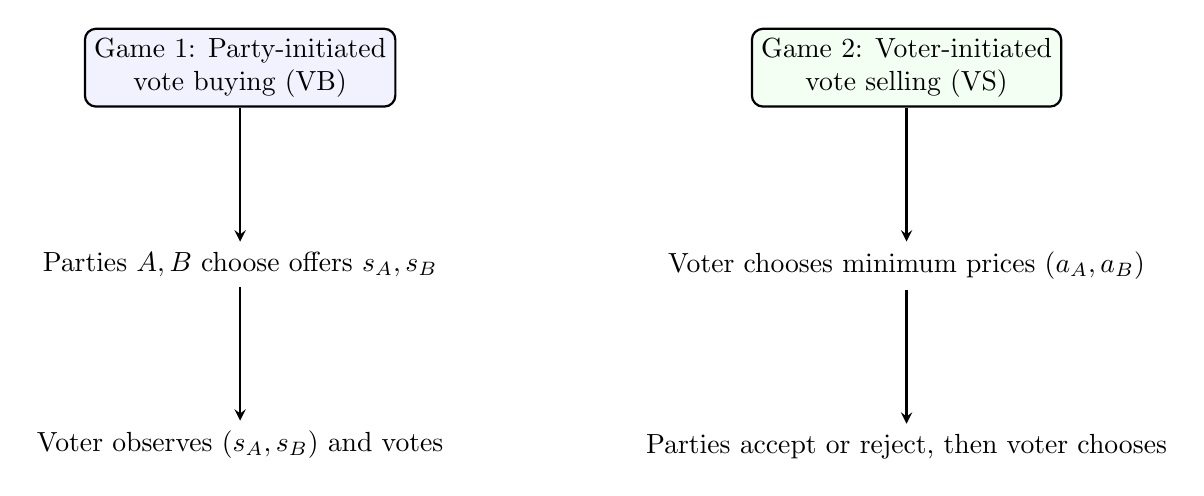
\begin{tikzpicture}[node distance=1.7cm,>=stealth,thick]
\node (vb) [rectangle,draw,rounded corners,align=center,fill=blue!5] {Game 1: Party-initiated \\ vote buying (VB)};
\node (vs) [rectangle,draw,rounded corners,align=center,fill=green!5,right=4.5cm of vb] {Game 2: Voter-initiated \\ vote selling (VS)};

\node (vb1) [below=of vb] {Parties $A,B$ choose offers $s_A,s_B$};
\node (vb2) [below=of vb1] {Voter observes $(s_A,s_B)$ and votes};

\node (vs1) [below=of vs] {Voter chooses minimum prices $(a_A,a_B)$};
\node (vs2) [below=of vs1] {Parties accept or reject, then voter chooses};

\draw[->] (vb) -- (vb1);
\draw[->] (vb1) -- (vb2);
\draw[->] (vs) -- (vs1);
\draw[->] (vs1) -- (vs2);
\end{tikzpicture}

\vspace{0.4cm}
\begin{itemize}
  \item \textbf{Same}: one pivotal voter, two parties, payoffs, budgets, electoral risk.
  \item \textbf{Different}: only \textbf{who moves first}, and thus who has bargaining leverage.
\end{itemize}
\end{frame}

\subsection{Key notation (light version)}

\begin{frame}[c]{Players, preferences, and stakes}
\begin{itemize}
  \item Parties $i \in \{A,B\}$ and one pivotal voter $j$.
  \item One-dimensional policy space: $\gamma \in \{1,\dots,100\}$ with $\gamma_A < \gamma_B$.
  \item Voter ideal point $x_j$; ideological utility if party $i$ wins:
  \[
  u_j(\gamma_i) = D - |x_j - \gamma_i|,\quad D>0.
  \]
  \item Preferred (core) party:
  \[
    i^\ast = \arg\max_{i \in \{A,B\}} u_j(\gamma_i).
  \]
  \item Ideological advantage of the core party:
  \[
    \Delta = u_j(\gamma_{i^\ast}) - u_j(\gamma_{-i^\ast}) > 0.
  \]
  \item $\Delta$ is the minimum compensating transfer needed to flip the vote.
\end{itemize}
\end{frame}

\begin{frame}[c]{Electoral risk and transfers}
\begin{itemize}
  \item Voter is pivotal with probability $\pi>0$.
  \item Party $i$ values winning at $W_i>0$; its electoral stake is
  \[
    R_i = \pi W_i.
  \]
  \item Think of $R_i$ as the maximum the party is willing to pay for the pivotal vote.
  \item Transfers:
  \begin{itemize}
    \item Vote buying: parties offer $s_i \ge 0$.
    \item Vote selling: voter requests $a_i \ge 0$.
  \end{itemize}
  \item Voter utility from voting for $i$ and receiving transfer $t_i$:
  \[
    U_j(i,t_i) = u_j(\gamma_i) + t_i.
  \]
\end{itemize}
\end{frame}

\subsection{Core logic of the model}

\begin{frame}[c]{Game 1: Party-initiated vote buying}
\begin{itemize}
  \item Parties observe $(x_j,\gamma_A,\gamma_B,R_A,R_B)$ and choose $s_i$ simultaneously.
  \item Voter observes $(s_A,s_B)$ and chooses a party.
  \item In a symmetric benchmark with $R_A=R_B=R$ and $R>\Delta$:
  \[
    s_{i^\ast}^{VB} = \Delta,\qquad s_{-i^\ast}^{VB} = 0.
  \]
  \item So:
  \begin{itemize}
    \item The ideologically preferred party buys the vote at the minimal compensating transfer.
    \item The opponent usually does not buy.
    \item Transfers concentrate on \textbf{core} supporters.
  \end{itemize}
\end{itemize}
\end{frame}

\begin{frame}[c]{Game 2: Voter-initiated vote selling}
\begin{itemize}
  \item Voter proposes $(a_A,a_B)$.
  \item Party $i$ accepts only if $a_i \le R_i$.
  \item Let $W$ be the \textbf{electorally stronger party} with $R_W>R_{-W}$.
  \item When $W$ is not the core party ($W \neq i^\ast$):
  \begin{itemize}
    \item There is a range of prices where both parties accept, but the voter prefers $W$.
    \item Voter can set $a_W$ close to $R_W$, extracting more from the electorally strong opponent.
  \end{itemize}
  \item Intuition: strong parties have higher stakes and higher willingness to pay; initiative lets voters try to exploit that.
\end{itemize}
\end{frame}

\begin{frame}[c]{Hypotheses}
\begin{itemize}
  \item \textbf{H1 (Core Targeting Under Party Initiative):}
  \begin{itemize}
    \item When parties initiate, transfers concentrate on ideologically proximate voters; parties mainly buy from their core.
  \end{itemize}
  \item \textbf{H2 (Selling to the Opponent Winning Party):}
  \begin{itemize}
    \item When voters initiate, they demand higher prices from electorally strong, often ideologically distant parties, using vote selling to hedge against electoral risk.
  \end{itemize}
  \item \textbf{H3 (Higher Voter Payoffs Under Party Initiative):}
  \begin{itemize}
    \item Because parties overspend under electoral risk when they initiate vote buying, while rejecting many high-priced proposals in vote selling, voters earn higher expected payoffs in VB than in VS.
  \end{itemize}
\end{itemize}
\end{frame}

%====================
% EXPERIMENT
%====================

\section{Experimental design}
\subsection{Setup and roles}

\begin{frame}[c]{Laboratory implementation}
\begin{itemize}
  \item \textbf{Subjects and implementation}
  \begin{itemize}
    \item 102 adult participants in a Chilean laboratory, implemented in \texttt{oTree}.
    \item Show-up fee plus performance-based earnings in experimental points.
  \end{itemize}
  \item \textbf{Roles}
  \begin{itemize}
    \item Each game: three real players (Party A, Party B, Voter).
    \item Each subject plays three independent games; for every game we fully re-randomize roles, ideology, budgets, and fictional vote shares.
  \end{itemize}
  \item \textbf{Information (common knowledge)}
  \begin{itemize}
    \item Voter's ideological payoffs if A or B wins.
    \item Party budgets.
    \item Fictional vote shares that determine whether the real voter is pivotal.
  \end{itemize}
\end{itemize}
\end{frame}

\begin{frame}[c]{Experimental flow}
\centering
\includegraphics[width=\textwidth]{/Users/hectorbahamonde/research/Exp_Vote_Selling/experimental_flow.pdf}

\vspace{0.2cm}
{\small Two institutional variants in an otherwise identical strategic environment.}
\end{frame}

\subsection{Ideology and electoral risk}

\begin{frame}[c]{Ideology, budgets, and pivotality}
\begin{itemize}
  \item \textbf{Ideology}
  \begin{itemize}
    \item Voter sees how many points she gets if A wins vs B wins.
    \item This implements $u_j(\gamma_A)$, $u_j(\gamma_B)$, and the ideological gap $\Delta$.
  \end{itemize}
  \item \textbf{Party budgets}
  \begin{itemize}
    \item Drawn at random and identical for both parties within a game.
    \item Constrain feasible offers and requested prices.
  \end{itemize}
  \item \textbf{Electoral risk}
  \begin{itemize}
    \item Fictional electorate of 3 or 5 additional voters.
    \item Vote shares for A and B imply safe vs close races.
    \item The real subject voter can be pivotal or not.
  \end{itemize}
\end{itemize}
\end{frame}

%====================
% EMPIRICAL RESULTS
%====================

\section{Empirical results}
\subsection{Behavior in the two games}

\begin{frame}[c]{Vote-buying offers vs vote-selling requests}
\centering
\includegraphics[width=\textwidth]{/Users/hectorbahamonde/research/Exp_Vote_Selling/depvarplot.png}
\vspace{0.2cm}

{\small Distributions of vote-buying offers (left) and vote-selling requests (right) as a share of party budgets.}
\end{frame}

\begin{frame}[c]{What the distributions suggest}
\begin{itemize}
  \item \textbf{Vote buying (VB):}
  \begin{itemize}
    \item Offers cluster at zero and at a small interior value around the compensating transfer $\Delta$.
    \item Consistent with the equilibrium where the core party buys and the opponent often offers nothing.
  \end{itemize}
  \item \textbf{Vote selling (VS):}
  \begin{itemize}
    \item Requested prices are widely dispersed.
    \item Many voters request very small transfers from at least one party.
    \item Others request amounts close to the party budget, especially when bargaining with electorally strong parties.
  \end{itemize}
  \item This motivates focusing on \textbf{pricing behavior} in VS to study how voters respond to ideology and electoral strength.
\end{itemize}
\end{frame}

\subsection{H1: Core targeting under party initiative}

\begin{frame}[c]{Modeling vote-buying offers}
\begin{itemize}
  \item Unit: party–voter dyad in the vote-buying game.
  \item We estimate:
  \[
    \text{Offer}_{di} = \gamma_0 + \gamma_1 \text{Ideology}_{di} + \gamma_2 \text{VoteShare}_{di} + \gamma_3 \text{Pivotal}_d + u_{di},
  \]
  using a linear model for positive offers.
  \item Complementary logit model for the probability of making \emph{any} offer.
  \item Standard errors clustered at the party level.
\end{itemize}
\end{frame}

\begin{frame}[c]{Results: parties target ideologically close voters}
\centering
\includegraphics[width=0.75\textwidth]{/Users/hectorbahamonde/research/Exp_Vote_Selling/H1_combined.png}
\vspace{0.2cm}

{\small Predicted offer size (left) and probability of any offer (right) as a function of ideological distance. Shaded regions: 95\% cluster-robust CIs.}
\end{frame}

\begin{frame}[c]{Interpreting H1}
\begin{itemize}
  \item As ideological distance increases:
  \begin{itemize}
    \item Parties offer \textbf{smaller} transfers.
    \item They are also less likely to make any offer at all.
  \end{itemize}
  \item When parties initiate the exchange, transfers concentrate on \textbf{ideologically proximate (core) voters}.
  \item This provides experimental support for \textbf{H1: Core Targeting Under Party Initiative}.
\end{itemize}
\end{frame}

\subsection{H2: Pricing the vote under voter initiative}

\begin{frame}[c]{Modeling requested prices (VS)}
\begin{itemize}
  \item Unit: voter–party dyad in the vote-selling game.
  \item Dependent variable:
  \[
    Y_{di} = \frac{a_{di}}{B_{di}} \times 100,
  \]
  requested price as a percentage of the party budget.
  \item Covariates:
  \begin{itemize}
    \item Ideological distance $\text{Ideology}_{di}$.
    \item Party vote share $\text{VoteShare}_{di}$ (electoral strength).
    \item Interaction $\text{Ideology}_{di} \times \text{VoteShare}_{di}$.
    \item Indicator for whether the real voter is pivotal.
  \end{itemize}
  \item Linear model with standard errors clustered by voter.
\end{itemize}
\end{frame}

\begin{frame}[c]{Requested prices by ideology and electoral strength}
\centering
\includegraphics[width=0.6\textwidth]{/Users/hectorbahamonde/research/Exp_Vote_Selling/m1plot.png}
\vspace{0.2cm}

{\small Predicted vote-selling prices by ideological distance for weak (20\%) and strong (80\%) parties. Shaded regions: 90\% cluster-robust CIs.}
\end{frame}

\begin{frame}[c]{Interpreting H2}
\begin{itemize}
  \item With \textbf{electorally weak} parties:
  \begin{itemize}
    \item Requested prices \textbf{decrease} with ideological distance.
    \item When the weak party is ideologically close, voters ask for relatively high transfers to insure against its likely loss.
    \item When it is distant, requested prices approach zero.
  \end{itemize}
  \item With \textbf{electorally strong} parties:
  \begin{itemize}
    \item Requested prices \textbf{increase} with ideological distance.
    \item When the strong party is distant, voters often escalate demands toward the party's full budget.
    \item Voters exploit stronger parties' higher electoral stakes $R_i$.
  \end{itemize}
  \item This pricing pattern is consistent with \textbf{H2}: when voters initiate, they use vote selling to hedge against electoral risk by demanding more from electorally strong, often ideologically distant parties.
\end{itemize}
\end{frame}

\subsection{H3: Who gains from each institution?}

\begin{frame}[c]{Payoffs by role and institutional variant}
\centering
\includegraphics[width=0.7\textwidth]{/Users/hectorbahamonde/research/Exp_Vote_Selling/payoffs_plot.png}
\vspace{0.2cm}

{\small Mean payoffs for voters and parties under party-initiated vote buying (VB) and voter-initiated vote selling (VS). Error bars: non-parametric 90\% CIs.}
\end{frame}

\begin{frame}[c]{Does initiative change who wins the game?}
\begin{itemize}
  \item \textbf{Parties:}
  \begin{itemize}
    \item Party payoffs are similar or slightly higher in VS than in VB.
    \item Shifting initiative to voters does not reduce party utilities in our setting.
  \end{itemize}
  \item \textbf{Voters:}
  \begin{itemize}
    \item Voters earn \textbf{higher average payoffs} when parties move first (VB) than when voters move first (VS).
    \item One-sided test of the difference in means is statistically significant (p-value from the t-test in the paper).
  \end{itemize}
  \item Interpretation:
  \begin{itemize}
    \item In VB, parties often overspend relative to the minimal compensating transfer $\Delta$, especially under electoral risk.
    \item In VS, very high requested prices are often rejected, leaving some voters with only ideological payoffs.
    \item Overall, initiative shapes how surplus is split: voters do better when parties initiate, while parties do at least as well when voters initiate.
  \end{itemize}
\end{itemize}
\end{frame}

%====================
% DISCUSSION
%====================

\section{Discussion}
\subsection{What we learn}

\begin{frame}[c]{Main takeaways}
\begin{itemize}
  \item Treating vote buying and vote selling as \textbf{institutional variants of the same market} clarifies:
  \begin{itemize}
    \item Who is targeted (core vs strong opponent).
    \item How much is paid.
    \item How surplus is allocated between parties and voters.
  \end{itemize}
  \item When \textbf{parties initiate} (VB):
  \begin{itemize}
    \item Transfers concentrate on core voters.
    \item Parties tend to overspend under electoral risk.
    \item Voters capture a larger share of surplus.
  \end{itemize}
  \item When \textbf{voters initiate} (VS):
  \begin{itemize}
    \item Voters demand higher prices from electorally strong, ideologically distant parties.
    \item Many of these high demands are rejected, lowering average voter payoffs.
    \item Parties' payoffs are stable or higher relative to VB.
  \end{itemize}
\end{itemize}
\end{frame}

\subsection{Implications and limits}

\begin{frame}[c]{Implications and next steps}
\begin{itemize}
  \item Conceptually:
  \begin{itemize}
    \item Clientelism is a \textbf{market} with both demand (parties) and supply (voters).
    \item Initiative is a core institutional rule that helps explain core–swing targeting and surplus allocation.
  \end{itemize}
  \item Methodologically:
  \begin{itemize}
    \item Experiments that vary who initiates the exchange can uncover mechanisms that are hard to see in observational data.
  \end{itemize}
  \item Limitations:
  \begin{itemize}
    \item One-shot lab games, no brokers, no repeated interactions or sanctions.
    \item Bilateral monopoly: two parties and one voter; no networks or groups of sellers.
  \end{itemize}
  \item Future work:
  \begin{itemize}
    \item Multi-voter and multi-party environments, with brokers and networks.
    \item Lab-in-the-field and survey experiments varying initiative.
    \item Linking this institutional perspective to ethnographic evidence on how often exchanges are party- vs voter-initiated.
  \end{itemize}
\end{itemize}
\end{frame}

%====================
% END
%====================

\miniframesoff
\begin{frame}[c]{Thank you}
\begin{center}
\vspace{-0.5cm}
\includegraphics[scale=0.05]{/Users/hectorbahamonde/research/Economic_Experiment_Vote_Selling/Resources_Presentation/qr-code.pdf}
\end{center}
\begin{itemize}
  \item Paper and abstract: {\color{blue}www.HectorBahamonde.com}
  \item Feedback very welcome.
\end{itemize}
\end{frame}

\end{document}
